%%%%%%%%%%%%%%%%%%%%%%%%%%%%%%%%%%%%%%%%%
% Beamer Presentation
% LaTeX Template
% Version 1.0 (10/11/12)
%
% This template has been downloaded from:
% http://www.LaTeXTemplates.com
%
% License:
% CC BY-NC-SA 3.0 (http://creativecommons.org/licenses/by-nc-sa/3.0/)
%
%%%%%%%%%%%%%%%%%%%%%%%%%%%%%%%%%%%%%%%%%

%----------------------------------------------------------------------------------------
%	PACKAGES AND THEMES
%----------------------------------------------------------------------------------------

\documentclass[10pt]{beamer}

\mode<presentation> {

% The Beamer class comes with a number of default slide themes
% which change the colors and layouts of slides. Below this is a list
% of all the themes, uncomment each in turn to see what they look like.

%\usetheme{default}
%\usetheme{AnnArbor}
%\usetheme{Antibes}
%\usetheme{Bergen}
%\usetheme{Berkeley}
%\usetheme{Berlin}
%\usetheme{Boadilla}
%\usetheme{CambridgeUS}
%\usetheme{Copenhagen}
%\usetheme{Darmstadt}
%\usetheme{Dresden}
%\usetheme{Frankfurt}
%\usetheme{Goettingen}
%\usetheme{Hannover}
%\usetheme{Ilmenau}
%\usetheme{JuanLesPins}
%\usetheme{Luebeck}
%\usetheme{Madrid}
\usetheme{Malmoe}
%\usetheme{Marburg}
%\usetheme{Montpellier}
%\usetheme{PaloAlto}
%\usetheme{Pittsburgh}
%\usetheme{Rochester}
%\usetheme{Singapore}
%\usetheme{Szeged}
%\usetheme{Warsaw}

% As well as themes, the Beamer class has a number of color themes
% for any slide theme. Uncomment each of these in turn to see how it
% changes the colors of your current slide theme.

\colorlet{beamer@blendedblue}{blue!40!black}
%\usecolortheme{albatross}
%\usecolortheme{beaver}
%\usecolortheme{beetle}
%\usecolortheme{crane}
%\usecolortheme{dolphin}
%\usecolortheme{dove}
%\usecolortheme{fly}
%\usecolortheme{lily}
%\usecolortheme{orchid}
%\usecolortheme{rose}
%\usecolortheme{seagull}
%\usecolortheme{seahorse}
%\usecolortheme{whale}
%\usecolortheme{wolverine}

%\setbeamertemplate{footline} % To remove the footer line in all slides uncomment this line
%\setbeamertemplate{footline}[page number] % To replace the footer line in all slides with a simple slide count uncomment this line

%\setbeamertemplate{navigation symbols}{} % To remove the navigation symbols from the bottom of all slides uncomment this line
}

\usepackage{graphicx} % Allows including images
\usepackage{booktabs} % Allows the use of \toprule, \midrule and \bottomrule in tables
\usepackage{algorithm}
\usepackage{algpseudocode}
\usepackage{multirow}
\usepackage{tikz}
\usepackage{xcolor} 
\usetikzlibrary{calc}
\usetikzlibrary{arrows,automata}
\usetikzlibrary{positioning}
\usetikzlibrary{decorations.text}
\usetikzlibrary{decorations.pathmorphing}
\usepackage[english]{babel}
\usepackage[utf8x]{inputenc}
\usepackage{amsmath}
\usepackage[colorinlistoftodos]{todonotes}
\usepackage{algorithm}
\usepackage{algpseudocode}
\usepackage{tikz}
\usetikzlibrary{tikzmark,calc}
\usepackage{mathtools}
\usepackage{amsthm}
\usepackage{subcaption,caption}
\usepackage{bm}
%\usepackage{enumitem}

\usepackage[english]{babel}

% \setlength{\parindent}{2em}
% \setlength{\parskip}{1em}
% \renewcommand{\baselinestretch}{1.6}
\DeclarePairedDelimiter\abs{\lvert}{\rvert}%

% to change colors
\newcommand{\fillcol}{green!10}
\newcommand{\bordercol}{black}
\newcommand\norm[1]{\left\lVert#1\right\rVert}

\newcommand\DrawBox[3][]{%
  \begin{tikzpicture}[remember picture,overlay]
    \draw[overlay,fill=gray!30,#1] 
    ([xshift=-8em,yshift=2.1ex]{pic cs:#2}) 
    rectangle 
    ([xshift=2pt,yshift=-0.7ex]pic cs:#3);
  \end{tikzpicture}%
}

\newcommand*{\captionsource}[2]{%
  \caption[{#1}]{%
    #1%
    \\\hspace{\linewidth}%
    \textbf{Source:} #2%
  }%
}

\DeclareMathOperator*{\argmax}{arg\,max}
\DeclareMathOperator*{\argmin}{arg\,min}
\DeclareMathOperator*{\minimize}{minimize}
\DeclareMathOperator*{\maximize}{maximize}


\algnewcommand\algorithmicinput{\textbf{Input:}}
\algnewcommand\INPUT{\item[\algorithmicinput]}

% \theoremstyle{definition}
% \newtheorem{definition}{Definition}[section]
\theoremstyle{remark}
\newtheorem{remark}{Remark}[section]
%----------------------------------------------------------------------------------------
%	TITLE PAGE
%----------------------------------------------------------------------------------------

\title[Introduction to Reinforcement learning]{Introduction to Reinforcement learning} % The short title appears at the bottom of every slide, the full title is only on the title page

\author{Tri Nguyen} % Your name
\institute[OSU] % Your institution as it will appear on the bottom of every slide, may be shorthand to save space
{
Summer Reading 2021 - Oregon State University \\ % Your institution for the title page
% \medskip
% \textit{lehoang@oregonstate.edu \endgraf } % Your email address
% }
}
\date{\today} % Date, can be changed to a custom date

\graphicspath{ {images/} }

\makeatletter
\renewcommand{\ALG@beginalgorithmic}{\footnotesize}
\makeatother

\newcounter{saveenumi}
\newcommand{\seti}{\setcounter{saveenumi}{\value{enumi}}}
\newcommand{\conti}{\setcounter{enumi}{\value{saveenumi}}}

\newcommand\numberthis{\addtocounter{equation}{1}\tag{\theequation}} % https://tex.stackexchange.com/questions/42726/align-but-show-one-equation-number-at-the-end 
\setbeamerfont{caption}{size=\scriptsize}
\setbeamertemplate{footline}[frame number]



\begin{document}
\DeclareFontShape{OT1}{cmss}{b}{n}{<->ssub * cmss/bx/n}{}
% \newtheorem{theorem}{Theorem}[section]
% \newtheorem{corollary}{Corollary}[theorem]
% \newtheorem{lemma}[theorem]{Lemma}
%------------------------------------------------
\begin{frame}
\titlepage % Print the title page as the first slide
\end{frame}
%------------------------------------------------
%------------------------------------------------

%------------------------------------------------
%\begin{frame}
%\frametitle{Contents} % Table of contents slide, comment this block out to remove it
%\tableofcontents % Throughout your presentation, if you choose to use \section{} and \subsection{} commands, these will automatically be printed on this slide as an overview of your presentation
%\end{frame}
%------------------------------------------------
%------------------------------------------------

%----------------------------------------------------------------------------------------
%	PRESENTATION SLIDES
%----------------------------------------------------------------------------------------


\begin{frame}
    \frametitle{RL Framework}
    \begin{figure}
        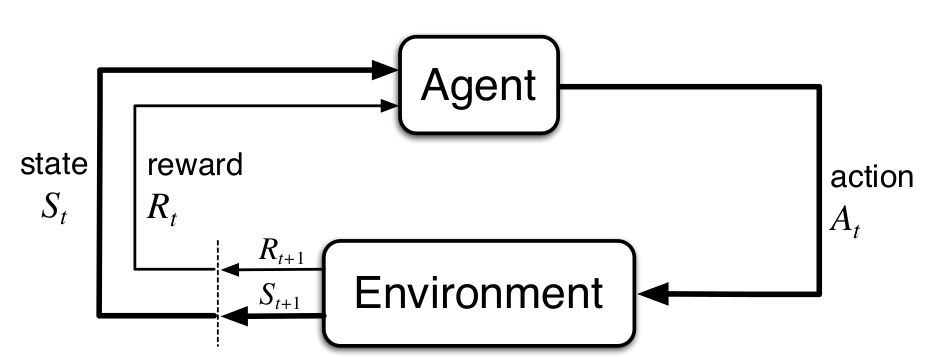
\includegraphics[width=0.4\textwidth]{figures/agent-environment.png}
   \end{figure}
   \textbf{Input of the framework}

   Environment - Agent interation:
   \begin{itemize}
       \item At time step $t$, \textit{agent} at state $S_t$ performs an action $A_t \in \mathcal{A}_t$
       \item { Environment's dynamics.} The \textit{environment} acts accordingly change to state $S_{t+1}$, emits a reward $R_{t+1}$
       \item { Episodic/Continuing task.} \textit{Return}: $G_t = \sum^{\infty}_{k=1} \gamma^{k}R_{t+k+1}$
   \end{itemize}
   \textbf{Output of the framework}

   {\color{blue} How.} An agent that acts on the environment so that it maximizes the expectation of \textit{return}, i.e., $ \mathbb{E}[G_t]$.
\end{frame}

\begin{frame}
\frametitle{Roadmap}
Given an MDP, find an optimal policy.
\begin{itemize}
    \item Policy Iteration
    \item Value Iteration
    \item Connection between 2 and variants
\end{itemize}
\end{frame}



\begin{frame}
    \frametitle{Environment's dynamics}
    Markov decision process (MDP) descibes environment's dynamics
   \begin{itemize}
       \item Finite sets of states, action, rewards $\mathcal{S}, \mathcal{A}, \mathcal{R}$
       \item Random variables $S_t \in \mathcal{S}, R_t \in \mathcal{R}$ are only dependent on preceding state and action, i.e.,
           $ p(s', r | s, a) \coloneqq \text{Pr}(S_t = s', R_t = r | S_{t-1} = s, A_{t-1} = a)$ 
       \item \textbf{Markov property.} State must include all information of the past that makes a difference for the future
   \end{itemize}
\end{frame}

\begin{frame}[t]
    \frametitle{Policy and Value Function}
    \begin{definition}
    \begin{itemize}
        \item Policy: $ \pi(a|s) = \text{Pr}(A_t =a| S_t = s)$
        \item Value function: 
            $ v_\pi(s) = \mathbb{E}_{\pi}[G_t | S_t =s] = \mathbb{E}_{\pi} \left[ R_{t+1} + \gamma G_{t+1} | S_t =s \right] $ 

        \item Action-value function: 
             $ q_\pi(s, a) = \mathbb{E}_{\pi} \left[ R_{t+1} + \gamma G_{t+1} | S_t=s, A_t=a \right] $ 

        \item Optimal policy: $\pi_{\ast}$ such that $v_{\pi_\ast}(s) \geq v_{\pi}(s)$ and for all $s \in \mathcal{S}$
        \item Optimal value function $v_{\pi_\ast}{s} =  $
    \end{itemize}
    \end{definition}
    \begin{remark}
        \begin{itemize}
            \item (Bellman equation) $v_\pi$ is the unique solution of
            \begin{equation*}
                 v_\pi(s) = \sum_{a} \pi(a|s) \sum_{s', r} p(s', r| S_t = s, A_t = a) \left( r + \gamma v_\pi(s') \right) 
            \end{equation*}
            \item (Bellman optimality equation) $v_{\ast}$ is the unique solution of
                \[
        \Rightarrow v_{\ast}(s) = \max_{a \in \mathcal{A}(s)} \; \sum_{s', r} p(s', r|  S_t =s, A_t = a)  \left( r + \gamma v_{\ast} (s') \right) \numberthis \label{eq:bellman_optim}
                \] 
        \end{itemize}
    \end{remark}
\end{frame}


\begin{frame}
    \frametitle{Policy Evaluation}
    % In order to find a treasure, we should know where we are
    Let $\bm{v} =
    \begin{bmatrix}
        v_\pi(s_1) & \ldots  & v_\pi(s_n)
    \end{bmatrix}^T  
    $,     \[
    \bm{R}  = \begin{bmatrix}
    \mathbb{E}[R_{t+1}| S_t = s_1] \\
    \ldots  \\
    \mathbb{E}[R_{t+1}| S_t = s_n] \\
    \end{bmatrix} , \quad
    \bm{P} = \begin{bmatrix}
        p(s_1 | s_1) & p(s_2 | s_1) & \ldots  & p(s_n | s_1) \\
        \ldots  \\
        p(s_1 | s_n) & p(s_2 | s_n) & \ldots  & p(s_n | s_n) \\
    \end{bmatrix} 
    \] 
\begin{align*}
    v_\pi(s) 
    &= \sum_{a} \pi(a|s) \sum_{s', r} p(s', r| S_t = s, A_t = a) \left( r + \gamma v_\pi(s') \right)  \\
    \Rightarrow \bm{v}_s &= \mathbb{E}_\pi [R_{t+1}| S_t = s] + \sum^{n}_{i=1} \gamma p(s_i | S_t = s)  \bm{v}_{s_i}
\end{align*} 

    Then Bellman equation in matrix form is
    \[
        \bm{v} = \bm{R} + \gamma \bm{P} \bm{v} 
    \] 
    \textit{Any method to solve a linear system can be used to find $\bm{v}$?}
\end{frame}

\begin{frame}
    \frametitle{Iterative Policy Evaluation}
    % \[
    %     \bm{v} = \bm{R} + \gamma \bm{P} \bm{v}, \text{define }T(\bm{v}) = \bm{R} + \gamma \bm{P} \bm{v} \Rightarrow T(\bm{v}) = \bm{v}
    % \] 
    \begin{itemize}
        \item Let $T(\bm{v}) = \bm{R} + \gamma \bm{P} \bm{v}$. By fixed-point property, a sequence $\bm{v}_k$ where  $\bm{v}_k = T(\bm{v}_{k-1})$ will converge to $\bm{v}_{\ast}$.
    \begin{figure}
        \centering
        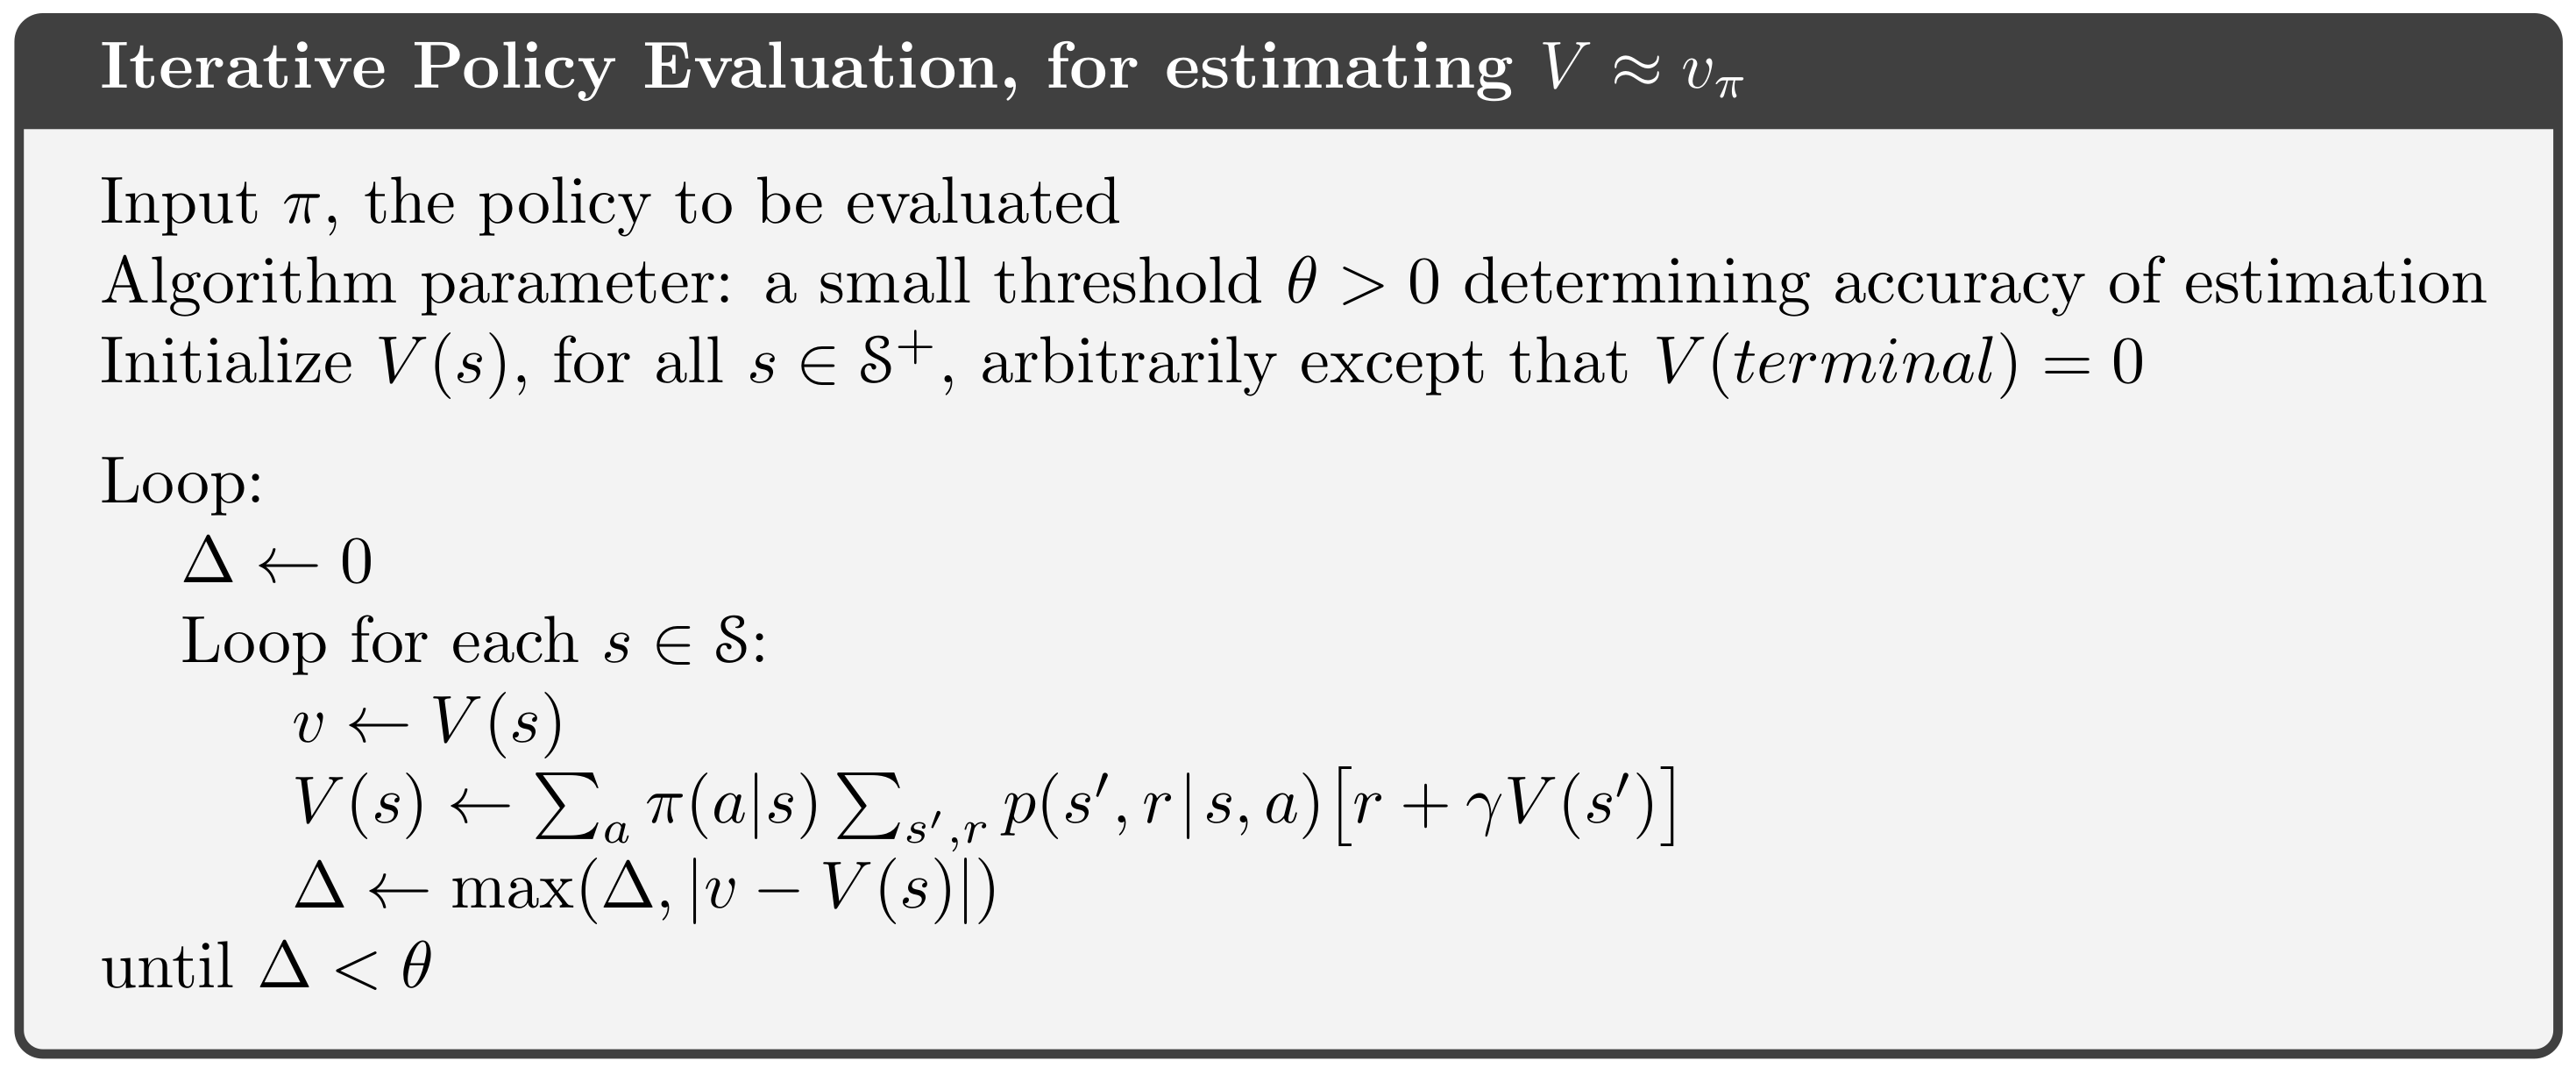
\includegraphics[width=0.7\textwidth]{figures/iterative_policy_evaluation.png}
    \end{figure}

        \item \textit{Expected updates}: In order to produce new $\bm{v}$, the algorithm updates value of every state
        \item \textit{In-place update}: Directly used new value of $v_\pi(s)$ during updating $v_\pi(s')$. . It is valid update since
         \[ \abs{T_{\pi}(\bm{v})[s] - T_{\pi}(\bm{v}')[s]} 
             \leq  \gamma \norm{ \bm{v} - \bm{v}' }_{\infty} \] 
    \end{itemize}
\end{frame}

\begin{frame}
    \frametitle{Policy Improvement}
    \begin{theorem}
        For 2 deterministic policy $\pi, \pi'$,  if for all $s \in \mathcal{S}$,
         \[
             q_\pi(s, \pi'(s)) \geq v_\pi(s) \Rightarrow \pi' \geq \pi
        \] 
    \end{theorem}
    Proof.
    \begin{align*}
        v_\pi(s) 
        &\leq q_\pi(s, \pi'(s)) \\
        &= \mathbb{E}_\pi \left[ R_{t+1} + \gamma v_\pi(S_{t+1}) | S_t = s, A_t = \pi'(s) \right] \\
        &= \mathbb{E}_{\pi'} \left[ R_{t+1} + \gamma v_\pi(S_{t+1}) | S_t = s \right] \\
        &\leq \mathbb{E}_{\pi'} \left[ R_{t+1} + \gamma q_\pi(S_{t+1}, \pi'(S_{t+1})) | S_t = s \right] \\
        &= \mathbb{E}_{\pi'} \left[ R_{t+1} + \gamma \mathbb{E}\left[ R_{t+2} + \gamma v_\pi(S_{t+2})| S_{t+1}, A_{t+1} = \pi'(S_{t+1}) \right] | S_t = s \right] \\
        &= \mathbb{E}_{\pi'} \left[ R_{t+1} + \gamma R_{t+2} + \gamma^2 v_\pi(S_{t+2}) | S_t = s \right] \\
        &\leq \ldots  \\
        &\leq \mathbb{E}_{\pi'} \left[ R_{t+1} + \gamma R_{t+2} + \gamma^{3}R_{t+3} + \ldots | S_t = s \right] \\
        &= v_{\pi'}(s)
    \end{align*}
\end{frame}

\begin{frame}
    \begin{itemize}
        \item Key to improvement is to find $\pi'$
    \begin{equation}
        q_\pi(s, \pi'(s)) \geq v_\pi(s)
    \end{equation} 
    \item Seek for an action to improve in short term (1 step)
    \begin{align*}
        \pi'(s) \coloneqq \argmax_{a} q_\pi(s, a)
    \end{align*}
    then by Policy improvement theorem, $\pi' \geq \pi$
    
\item If no improvement is available, i.e., $v_\pi = v_{\pi'}$ then $v_\pi = v_\ast$ because
    \begin{align*}
        v_{\pi'}(s) 
        &= \max_{a} \mathbb{E}[R_{t+1} + \gamma v_{\pi} (s) |S_t = s, A_t=a] \\
        &= \max_{a} \mathbb{E}[R_{t+1} + \gamma v_{\pi'} (s) |S_t = s, A_t=a]
    \end{align*}
    
\item Note that $v_\pi = v_{\pi'}$  but not $\pi = \pi'$ gives a hint about reaching optimal value.
    \end{itemize}
\end{frame}

\begin{frame}
    \frametitle{Policy Iteration}
    \[
        \pi_0 \xrightarrow{\text{Eval} } v_{\pi_0} \xrightarrow{\text{Improve} } \pi_1 \xrightarrow{\text{Eval} } v_{\pi_1} \xrightarrow{\text{Improve}} \ldots  \xrightarrow{\text{Improve} } \pi_{\ast} \xrightarrow{\text{Eval} } v_{\pi_{\ast}}
    \] 
    \begin{figure}
        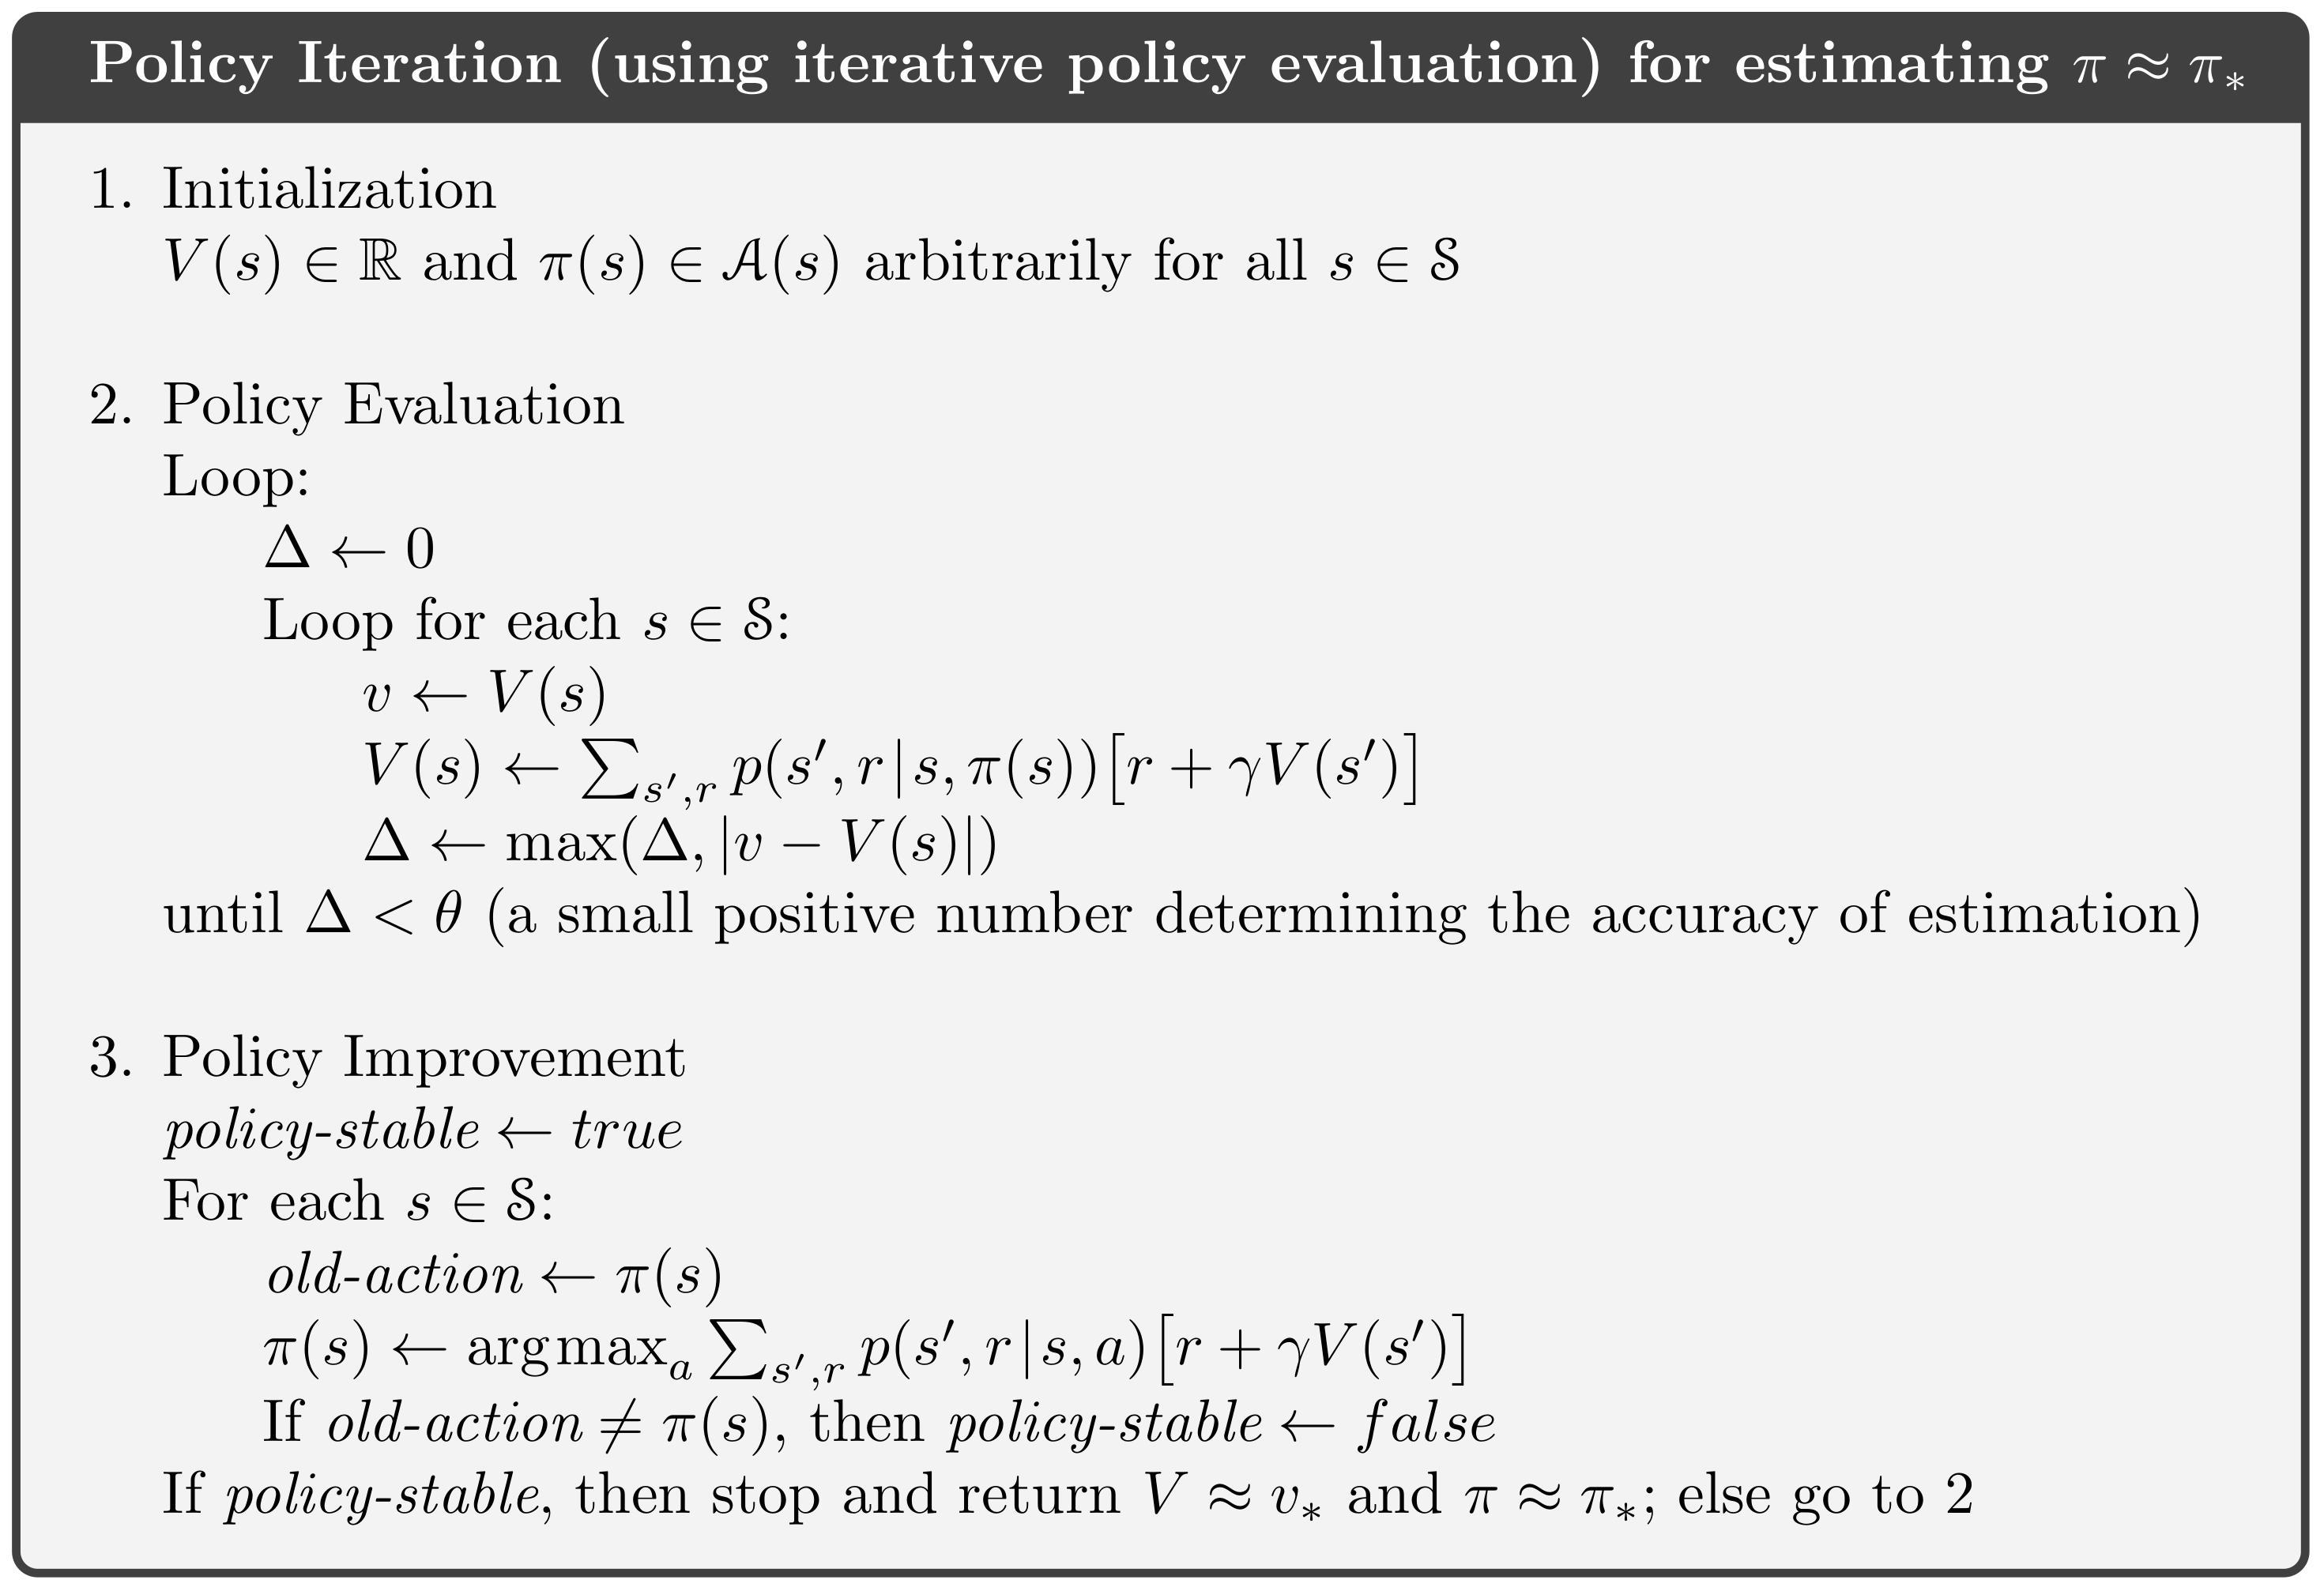
\includegraphics[width=0.65\textwidth]{figures/policy_iteration.png}
        \caption{There's a subtle bug}
    \end{figure}

    \begin{itemize}
        \item Truncated variant: run a small $K$ number of iterations for step 2.
        \item Converge very fast in few iterations, but computationally expensive because of policy evaluation
    \end{itemize}
\end{frame}

% \begin{frame}
%     \frametitle{Policy Iteration}
%     \begin{figure}
%         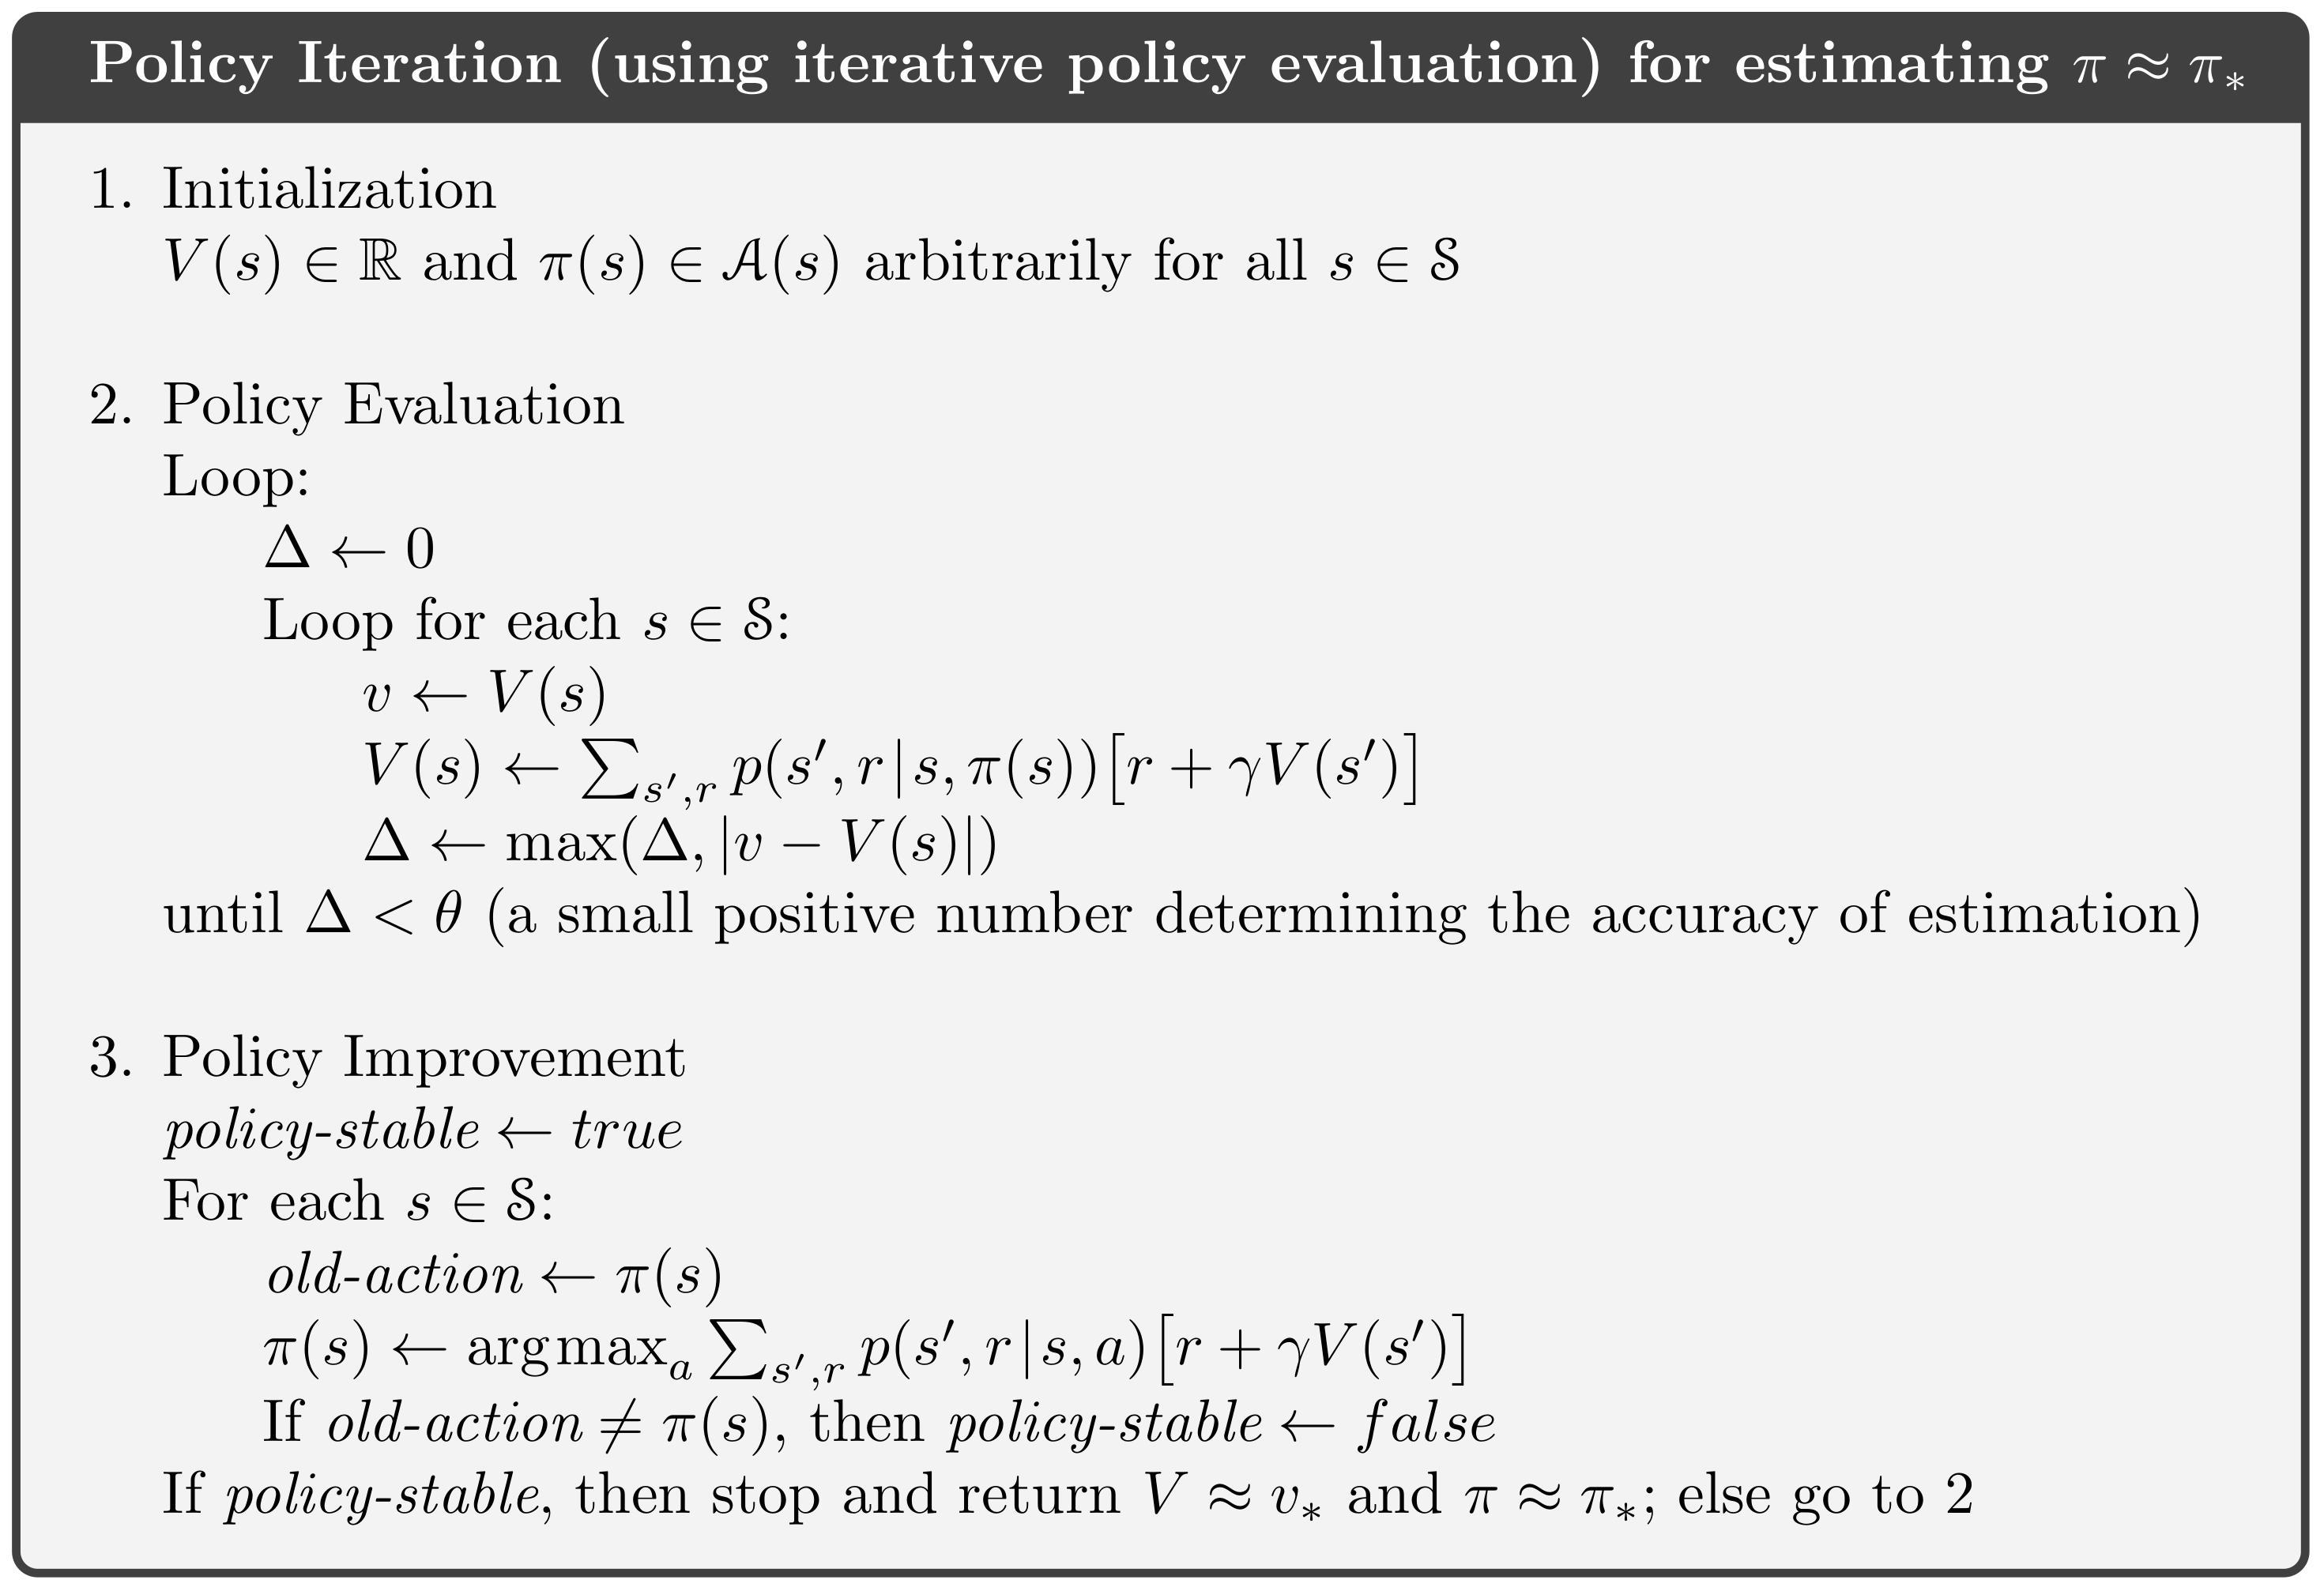
\includegraphics[width=0.65\textwidth]{figures/policy_iteration.png}
%     \end{figure}
% \end{frame}

\begin{frame}
    \frametitle{Value Iteration}
    Combine policy improvement and truncated policy evalution in one step:
    \begin{equation}
        v_{k+1}(s) \coloneqq \max_{a} \; \mathbb{E} [R_{t+1} + \gamma v_{k}(S_{t+1}) | S_t = s, A_t = a]
        \label{eq:vi}
    \end{equation} 
    \begin{itemize}
        \item Truncated policy evaluation: Vanilla policy evalution with only 1 iteration
        \item (\ref{eq:vi}) is Bellman optimality equation if substituting $v_k, v_{k+1}$ by $v_\ast$
    \begin{figure}
        \centering
        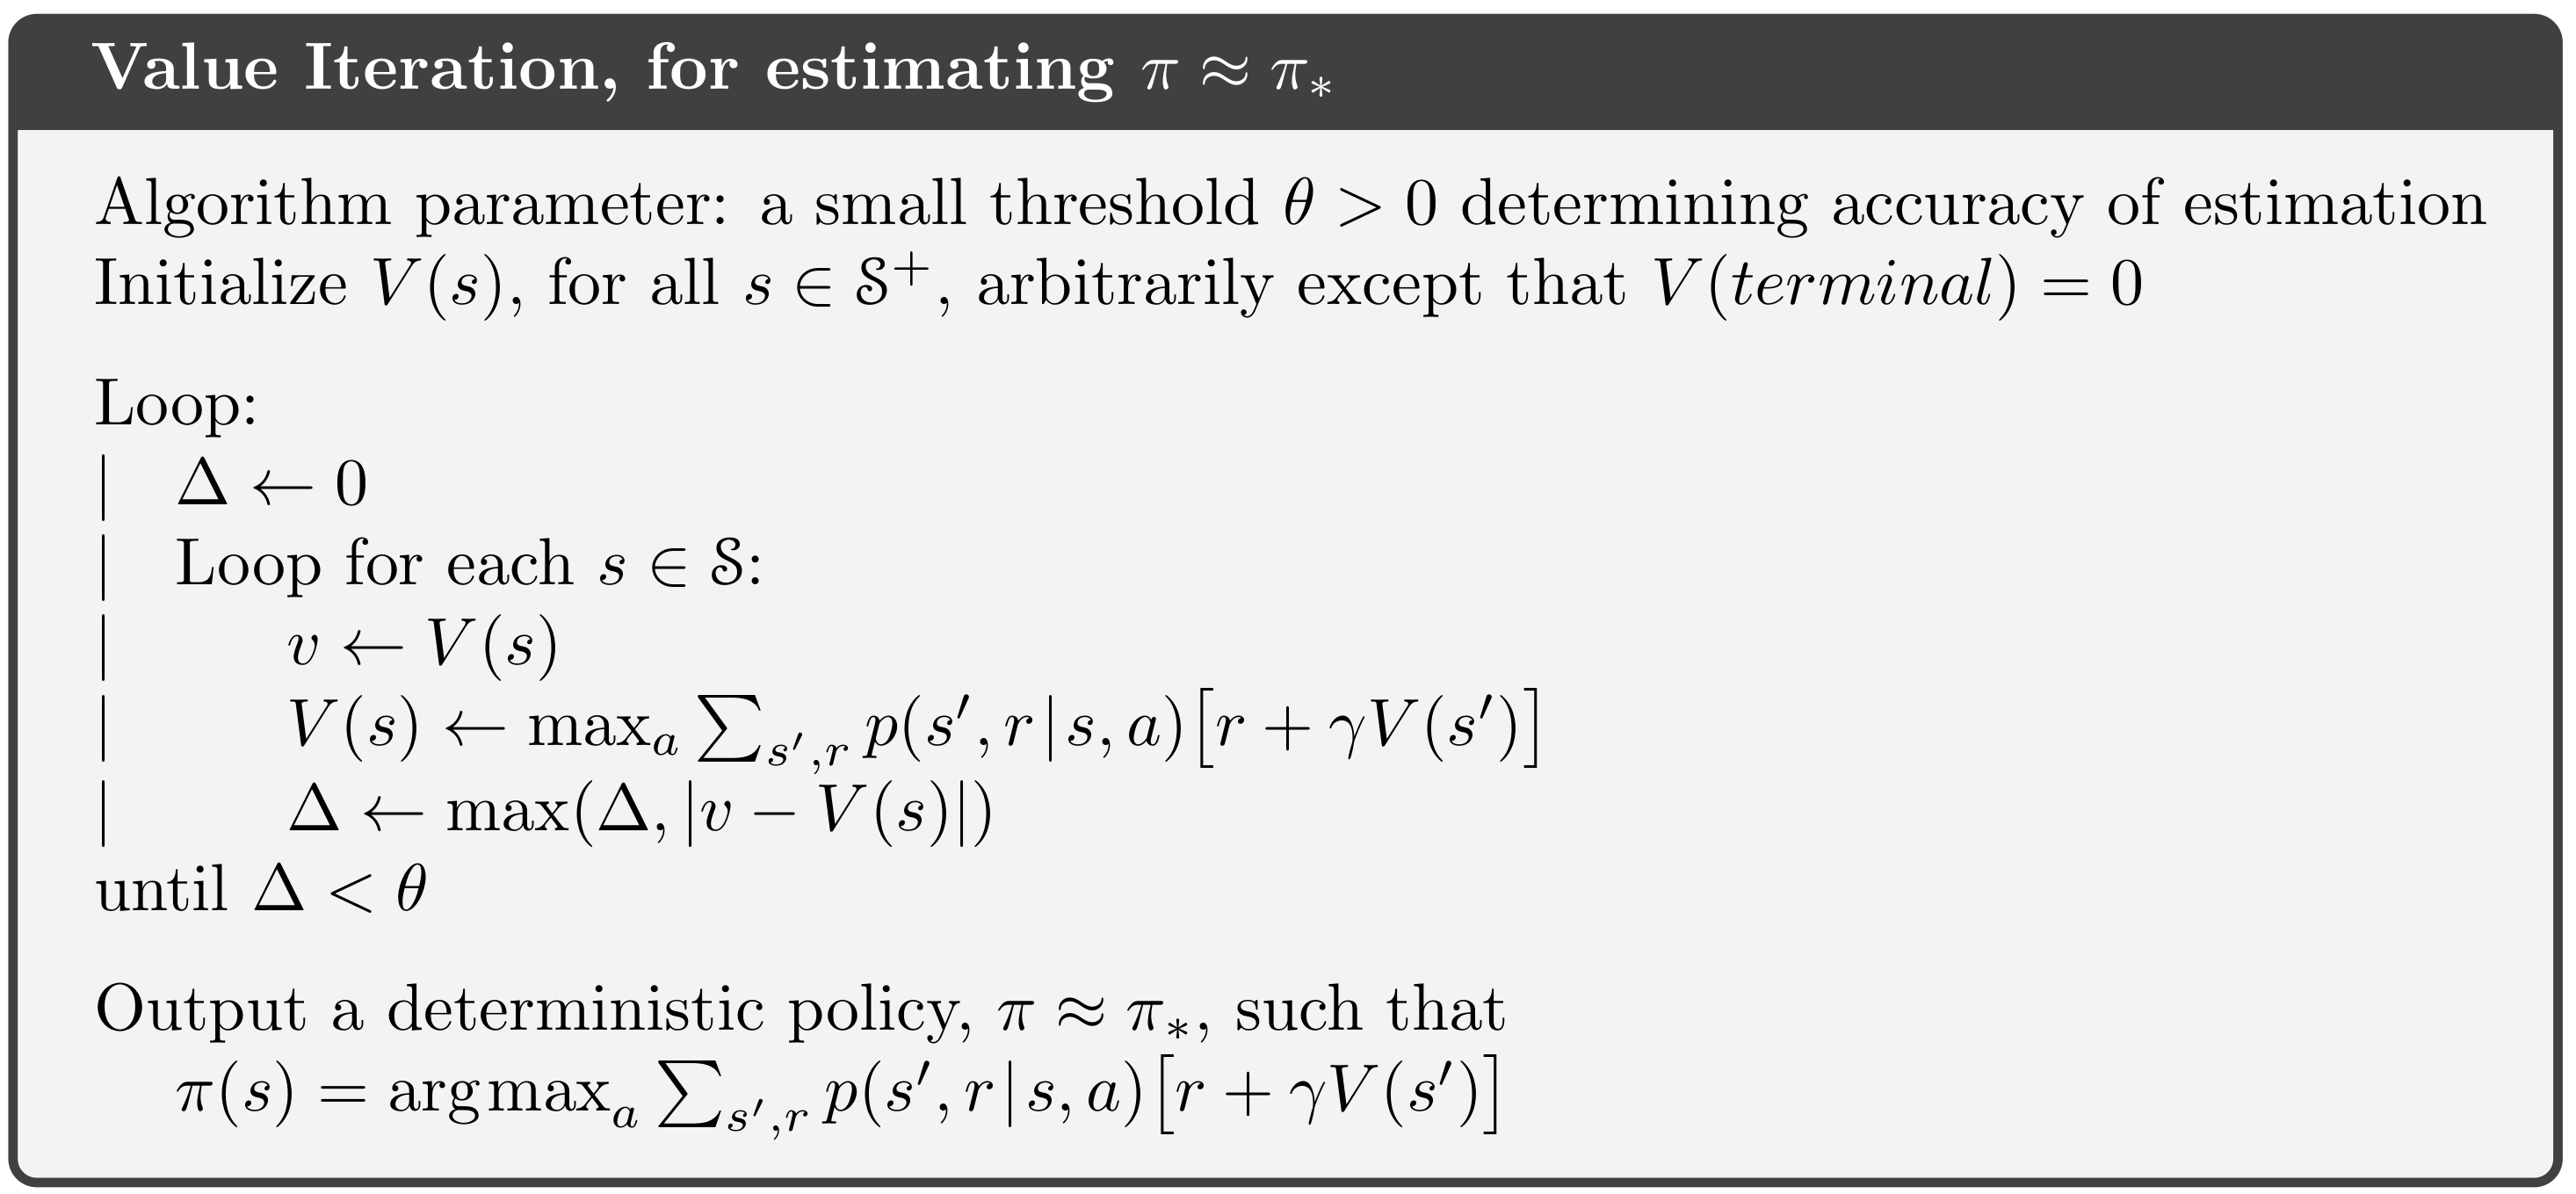
\includegraphics[width=0.65\textwidth]{figures/value_iteration.png}
    \end{figure}
\item The inner loop does not neccessarily need to run over all $s \in \mathcal{S}$ (\textit{Asynchronous DP})
    \end{itemize}
\end{frame}




\begin{frame}
    \frametitle{Generalized Policy Iteration}
    \begin{figure}
        \centering
        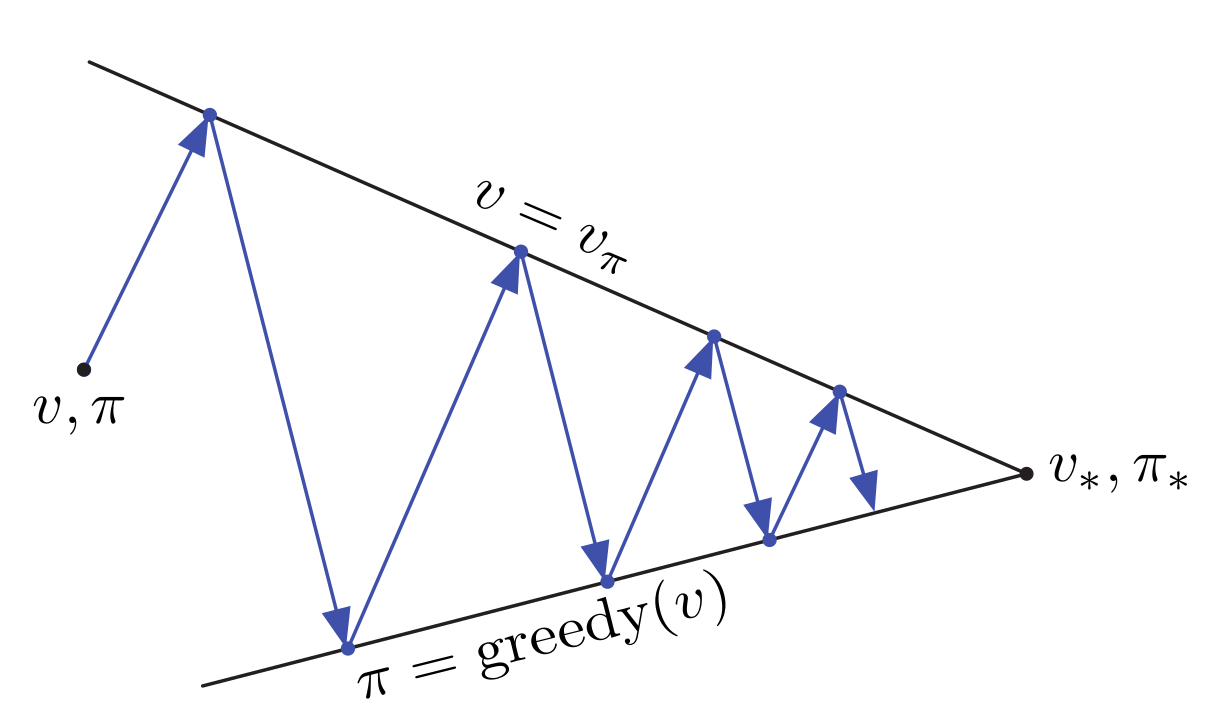
\includegraphics[width=0.5\textwidth]{figures/generalized_PI.png}
    \end{figure}
    There's is a notion of alternating between policy evaluation and policy improvement
    \begin{itemize}
        \item In PI, a policy improvement is performed after a completing policy evaluation and vice versa.
        \item In VI, only single iteration of policy evaluation is performed in between each policy improvement.
        \item We can even interleaved at finer grain: mixed asynchronous DP in VI with PI
        \item Policy evaluation and policy improvement are both competing and coorperating.
    \end{itemize}
\end{frame}


\begingroup
\small% \small in 11pt base font is 10pt
\begin{frame}
    % Then Bellman equation in matrix form is
    % \[
    %     v = R + \gamma P v  \Rightarrow v = (I - \gamma P)^{-1} R
    % \]

    \begin{figure}
        \begin{subfigure}{0.38\textwidth}
            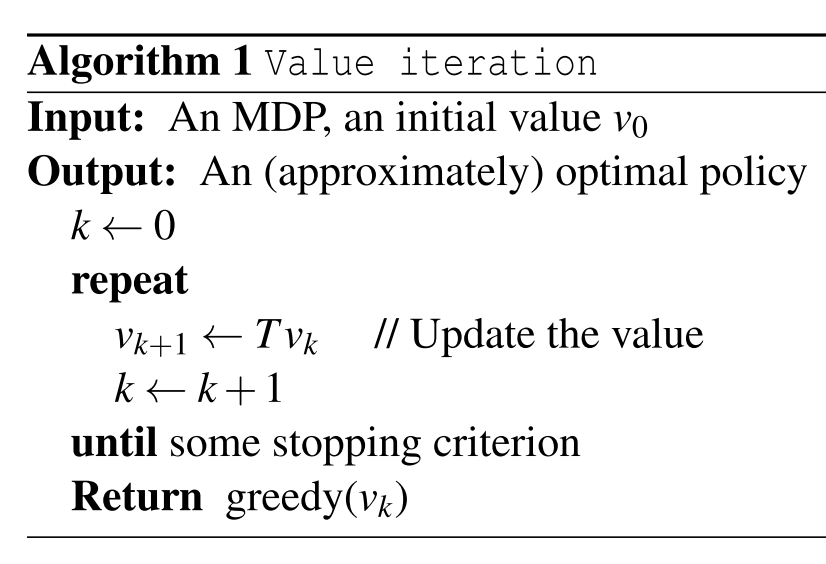
\includegraphics[width=\textwidth]{figures/VI_summary.png}
        \end{subfigure}
        \begin{subfigure}{0.45\textwidth}
            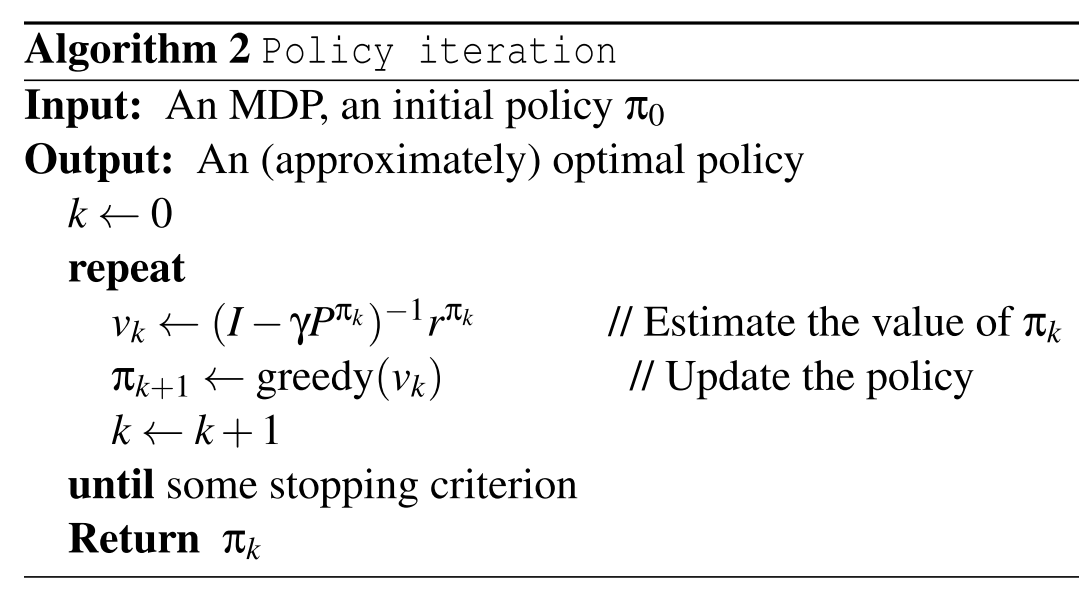
\includegraphics[width=\textwidth]{figures/PI_summary.png}
        \end{subfigure}
        \caption{$v = R + \gamma P v  \Rightarrow v = (I - \gamma P)^{-1} R$}
    \end{figure}
    {
        \scriptsize
        Define
        \begin{align*}
            T_{\pi}(v)[s] &\coloneqq \sum_{a} \pi(a|s) \sum_{s', r} p(s', r| S_t = s, A_t = a) \left( r + \gamma v_\pi(s') \right)  \\
        T(v)[s] &\coloneqq \max_{a \in \mathcal{A}(s)} \; \sum_{s', r} p(s', r|  S_t =s, A_t = a)  \left( r + \gamma v_{\ast} (s') \right)
        \end{align*} 
    }

    \begin{itemize}
        \item Value iteration
    \[
    \begin{cases}
        \pi_{k+1} \leftarrow \text{greedy}(v_{\pi_k}) \\
        v_{k+1} \leftarrow T_{\pi_{k+1}}(v_{k}) \\
    \end{cases}
    \Leftrightarrow
    \begin{cases}
        \pi_{k+1} \leftarrow \text{greedy}(v_{\pi_k}) \\
        v_{k+1} \leftarrow R + \gamma P v_{k} \\
    \end{cases}
    \] 
\item Policy iteration
    \[
    \begin{cases}
        \pi_{k+1} \leftarrow \text{greedy}(v_{\pi_k}) \\
        v_{k+1} \leftarrow T_{\pi_{k+1}}^{\infty}(v_{k}) \\
    \end{cases}
    \Leftrightarrow
    \begin{cases}
        \pi_{k+1} \leftarrow \text{greedy}(v_{\pi_k}) \\
        v_{k+1} \leftarrow (I - \gamma P)^{-1}R \\
    \end{cases}
    \] 
    \end{itemize}
\end{frame}

\begin{frame}
    \begin{itemize}
        \item Bertsekas and Ioffe (1996) introduced an operator which is proved to be a $\lambda \gamma$-contraction respect to $l_\infty$ norm
    \begin{align*}
        M_k(v) 
        &\coloneqq  (1 - \lambda) T_{\pi_{k+1}} (v_k) + \lambda T_{\pi_{k+1}} (v) \\
        &=  (1 - \lambda) (R + \gamma P v_k) + \lambda (R + \gamma P v) \\
        &=  R + (1-\lambda) \gamma P v_k + \lambda \gamma P v
    \end{align*} 
\item Since $M_k(v)$ is a contraction, it has a unique fixed point, $v_{M} = M_k^{\infty}(v)$ exists
    \begin{align*}
        v_{M} &= R + (1- \lambda)\gamma P v_k + \lambda \gamma P v_M  \\
        \Leftrightarrow v_M &= (I - \lambda \gamma P)^{-1} (R + (1 - \lambda) \gamma P v_k)
    \end{align*} 
\item Use $M_k(v)$, $\lambda$ policy iteration's update is given by.
    \begin{align*}
    \begin{cases}
        \pi_{k+1} \leftarrow \text{greedy}(v_{\pi_k}) \\
        v_{k+1} \leftarrow (I - \lambda \gamma P)^{-1} (R + (1 - \lambda) \gamma P v_k) 
    \end{cases}
    \end{align*} 
    \item Let $T_\lambda(v) := v_M = (I - \lambda \gamma P)^{-1} (R + (1 - \lambda) \gamma P v_k)$ be operator.
    \begin{align*}
    \begin{cases}
        \pi_{k+1} \leftarrow \text{greedy}(v_{\pi_k}) \\
        v_{k+1} \leftarrow T_\lambda (v_k) 
    \end{cases}
    \end{align*} 
    \end{itemize}
\end{frame}

\begin{frame}
    \begin{itemize}
        \item In the updating step, $\lambda$ policy iteration trying to find fixed point of operator $M_k(v)$. 
        \item Define a sequence of $v_1, v_2, \ldots $ such as $v_{j+1} = M_k(v_j)$
            We have:
            \begin{align*}
                v_{j+1} = M_k(v_j) 
                &= (1- \lambda) T_{\pi_{k+1}}(v_k) + \lambda T_{\pi_{k+1}}(v_j) \\
                &= (1- \lambda) T_{\pi_{k+1}}(v_k) + \lambda T_{\pi_{k+1}}(M_k(v_{j-1})) \\
                &= (1- \lambda) T_{\pi_{k+1}}(v_k) + \lambda T_{\pi_{k+1}}\left( (1-\lambda) T_{\pi_{k+1}}(v_k) + \lambda T_{\pi_{k+1}} (v_{j-1}) \right) \\
                &= (1- \lambda) (T_{\pi_{k+1}}(v_k) + \lambda T_{\pi_{k+1}}^2 (v_k)) + \lambda^2 T_{\pi_{k+1}}^2 T_{\pi_{k+1}} (v_{j-1}) ) \\
                &= \ldots  \\
                &= (1- \lambda) \sum^{\infty}_{j=0} \lambda^{j} T_{\pi_{k+1}}^{j+1} (v_k)
            \end{align*}
    \begin{align*}
        \text{so that the update rule becomes}
    \begin{cases}
        \pi_{k+1} \leftarrow \text{greedy}(v_{\pi_k}) \\
        v_{k+1} \leftarrow (1- \lambda) \sum^{\infty}_{j=0} \lambda^{j} T_{\pi_{k+1}}^{j+1} v_k  
    \end{cases}
    \end{align*} 
    % The last equation comes from the fact that
    % \[
    %     v_m = (1- \lambda) T_{\pi_{k+1}}(v_k) + \lambda (R + \gamma P v_{k})
    % \] 
    % \item Let $T_\lambda(v) := v_M = (I - \lambda \gamma P)^{-1} (R + (1 - \lambda) \gamma P v_k)$ be another operator.
    % \begin{figure}
    %     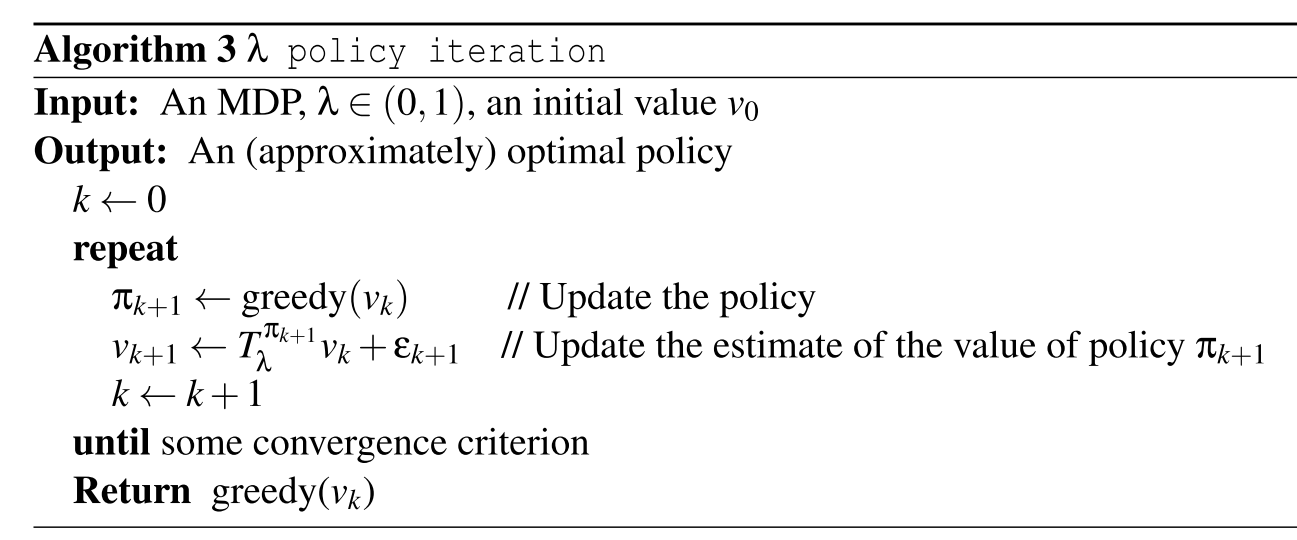
\includegraphics[width=0.5\textwidth]{figures/lambda_PI.png}
    % \end{figure}
    %
    \end{itemize}
\end{frame}

\begin{frame}
    \frametitle{Summary}
    \begin{itemize}
        \item Policy evaluation is based on Bellman equation
        \item Value iteration is based on Bellman optimality equation
        \item GPI views a different levels of interleaving between policy evaluation and policy improvement
    \end{itemize}
\end{frame}

\end{document}

